\chapter{Cost-aware fleet scheduling and model routing}\label{cost-aware-fleet-scheduling-and-model-routing}

A fleet can raise throughput while raising the cost of each accepted result, and only the fleet's own traces can establish whether it did. Concurrent execution, together with the willingness to take on work a human team would have left queued, exposes more work to model inference, review, and recovery. Throughput alone therefore does not establish the economic result.

The evidence for changing that outcome is thin, and most of it is transferred from other fields. This chapter has one strong software-engineering result about cheap baselines, directional literature from observatory and compute-cluster scheduling, and my own fleet replay, which is narrative illustration with no independent evidentiary weight. The relevant evidence cluster has one strong item rather than zero.

Astronomical observation scheduling is the dominant transfer domain, in two forms: a survey telescope's nightly planner, and a gravitational-wave follow-up scheduler built on the same facility. Learned compute-cluster scheduling is the second domain and search-based software engineering the third. Budget-constrained bandit theory and router calibration cover the routing decision alone rather than a complete fleet.

These are schedulers for telescopes and compute clusters. None of the cited works claims results for software agent fleets. The decision architecture transfers: re-decide from current state, cap the time spent deciding, compare against cheap alternatives, and preserve enough measurement to detect a bad policy. Cadence, threshold, cost ratio, and performance constants do not transfer with it.

Allocation policy is easy to mistake for a local configuration choice. In an agent fleet, the policy determines which model receives a request, which queued item moves first, whether running work remains fixed, and when the system discards an obsolete plan. These choices couple inference cost to elapsed time, reviewer load, and the probability that completed work will survive evaluation. A repair loop can consume the savings from a cheaper call. A schedule that is better on paper is not better in operation if computing it delays the work past its deadline. I therefore treat scheduling and routing as decisions under measurement.

\section{Name the decision before reaching for the algorithm}\label{name-the-decision-before-reaching-for-the-algorithm}

Cheapest-sufficient routing means choosing, for each task, the least expensive worker predicted to meet that task's declared requirement. The worker may be a model tier, a model-plus-tool configuration, or another execution pool with a known price. The important word is sufficient. The router is not minimizing the invoice in isolation, and it is not assigning every task class to a model through a hand-written rule. It estimates expected performance and expected cost for the request in front of it, then chooses the lowest-cost option that satisfies the stated tradeoff. This definition leaves open how performance is predicted and how sufficiency is expressed. These are deployment decisions with consequences for calibration and evaluation.

Shipping the incumbent at the deadline means placing a hard time cap on schedule computation and executing the best feasible plan available when the cap expires. A feasible plan respects the constraints that cannot be violated, such as capacity, deadlines treated as hard, and work already in flight. The incumbent is the best such plan found so far. Waiting longer may find a better plan or prove that the current one is optimal, but the schedule has operational value only while it describes a world that still exists. With a cap, decision latency is chosen rather than discovered.

The optimality gap records how far the shipped solution might be from the best possible one, using the best bound known when the cap was reached. The gap retains information about the remaining uncertainty in solution quality. Shipping an incumbent without its gap records two different states as one: a plan known to be nearly best, and a merely feasible plan found before the search made much progress. Operations may reasonably execute both. Evaluation should not treat them as equivalent.

\begin{figure}
\centering
\pandocbounded{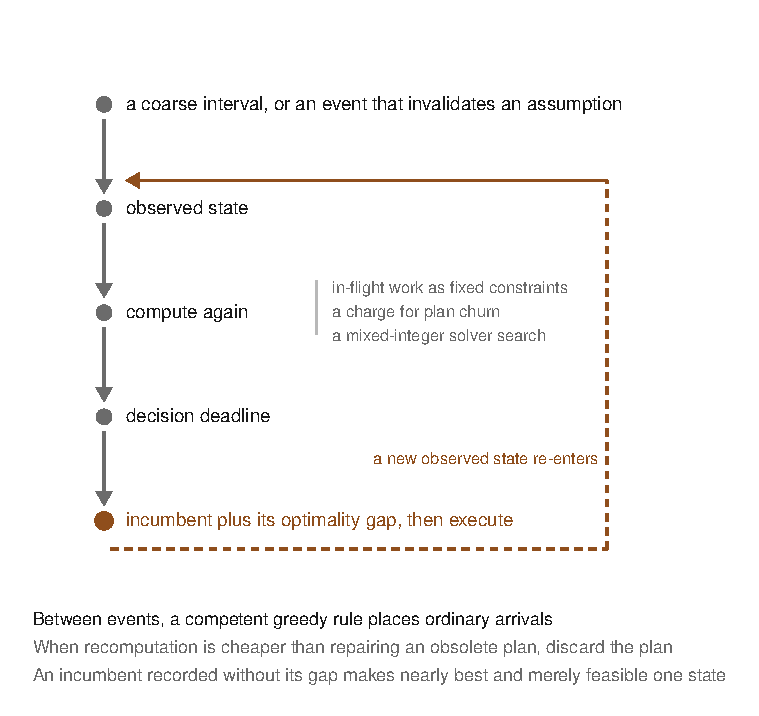
\includegraphics[keepaspectratio,alt={The re-decision loop recomputes from observed events under fixed work and churn costs, then executes a deadline capped incumbent while retaining its optimality gap.}]{figures/ch18-redecision-loop.pdf}}
\caption{The re-decision loop recomputes from observed events under fixed work and churn costs, then executes a deadline capped incumbent while retaining its optimality gap.}
\end{figure}

Ordinary arrivals remain greedy between events, and the plan is discarded only when fresh optimization costs less than repairing obsolete work.

These terms specify decisions. A fleet operator needs to decide what counts as sufficient, how long schedule computation may run, which constraints are inviolable, and what quality information must survive execution. The companion catalog contains the algorithmic patterns. The narrower question here is whether these decisions produce lower cost or more reliable flow on the fleet's own workload.

\section{Re-decide cheaply and ship the incumbent}\label{re-decide-cheaply-and-ship-the-incumbent}

An observatory scheduler can spend the night improving a plan that clouds have already invalidated, or it can compute another imperfect plan from the sky it can still observe. Bellm et al.~(\href{https://arxiv.org/abs/1905.02209}{2019}) described the Zwicky Transient Facility taking the second approach, in production since 2018. It re-solves its nightly integer program when conditions invalidate the schedule instead of enumerating weather scenarios in advance. The support for transferring this choice to agent fleets is three directional literature items from observatory scheduling, with no strong result and no software-fleet measurement among them. The recommendation is therefore limited to choosing and measuring a re-decision policy. The cadence remains an agent-fleet deployment decision.

The schedule should be treated as the current output of a control loop. At a coarse interval, or after an event that invalidates an important assumption, the scheduler computes again from observed state. Between those events, a competent greedy rule can place ordinary arrivals without paying the cost of a full solve. If recomputation is cheaper than repairing an obsolete plan, the obsolete plan should be discarded. The comparison must include decision latency. An excellent schedule delivered after the queue has changed is a schedule for a fleet that no longer exists.

Current state includes more than the queue. Running work consumes capacity, may hold a repository lease or a review slot, and may have produced state that another worker cannot cheaply reconstruct. A re-solve should represent that in-flight work as fixed constraints unless preemption has been separately justified. It should also charge for plan churn, meaning avoidable reassignment or resequencing that makes workers discard useful preparation. The companion-catalog pattern \texttt{design-the-online-rescheduling-loop} treats cadence, invalidation triggers, and this churn penalty as parts of the scheduling algorithm. They are not operational details to add after selecting an objective.

At the decision deadline, execute the mixed-integer solver's incumbent and record its optimality gap. This prescription follows from the mismatch between proof time and operational time. Solvers often find a feasible plan before they finish establishing how close it is to the best plan, while new arrivals and changing capacity continue to age the state on which that plan was built. The cap prevents schedule computation from becoming another queue. The stored gap makes later analysis possible. Operators can then ask whether large gaps coincide with worse flow, whether more solve time would have changed executed choices, and whether a simpler rule performs just as well.

Parazin et al.~(\href{https://arxiv.org/abs/2203.00013}{2022}) measured a mixed-integer scheduler for gravitational-wave follow-up against a tuned greedy heuristic, and neither method won outright. At a 500-second cap, their scheduler and the gwemopt heuristic each did better on different skymaps, and only 37 of 97 well-localized skymaps improved under the optimization comparison the paper reported. Across 951 simulated events, the headline result favored a hybrid of the two by roughly 3 to 11 percent in detection efficiency. A 100-second cap, they reported, would have truncated only 64 more schedules without substantial efficiency loss.

These figures are directional evidence from a gravitational-wave follow-up workload rather than fleet parameters. They support measuring the cap, the gap, and a hybrid, each against a tuned simple rule. They also argue against assuming in advance that either the optimizer or the simple rule will win.

Naghib et al.~(\href{https://arxiv.org/abs/1810.04815}{2019}) described a second observatory design that makes the same point about state: a feature-based, memoryless policy that decides again at every step from current state. `Memoryless' here does not mean that the system forgets durable facts. It means that the next scheduling choice does not depend on preserving a brittle sequence of earlier planned choices. Interruptions are absorbed when the scheduler observes the new state and makes another decision. Their evidence comes from a framework and a simulation. It therefore establishes a plausible architecture rather than a measured benefit for agent execution.

The global problem and the local problem should remain distinct. A fleet-wide allocator decides how scarce model tiers, reviewers, or execution pools are divided across work. A per-worker dispatcher decides which eligible item a particular worker takes next. The companion catalog records this as \texttt{split-fleet-scheduling-into-global-and-local-levels}. Combining both decisions in one opaque score makes it difficult to determine whether a bad outcome came from resource allocation or queue order. It can also cause local dispatch to undo a capacity decision that the global layer just made.

There is a more ambitious companion pattern, \texttt{formalize-work-as-constraints-and-solve-globally}, whose cataloged lineage reaches Hubble scheduling in 1990. It proposes expressing work requests in one constraint language so the allocator can solve across them. This architecture is useful only if the request representation captures the constraints that operations actually enforce. A nominally global solution built from incomplete deadlines, missing affinity constraints, or false independence assumptions can be less coherent than separate local rules. \texttt{audit-the-allocation-layer} is therefore marked as an aside in the catalog: name the execution, planning, and optimization levels, then inspect which policy actually dispatches work. Its observatory analogy has no software-side measurement.

Probe costs belong in the same accounting. The thin-support aside \texttt{probe-only-above-an-uncertainty-threshold} asks whether a dry run, canary, or classifier call can reduce enough uncertainty to repay its cost. Its theory comes from adversarial single-machine scheduling. Its constant therefore does not transfer. The usable question is local: for which uncertain requests does a probe change the chosen worker or the schedule often enough to justify the extra latency and inference? If that answer cannot be recovered from logs, probing is another unmeasured policy.

This decision has an explicit boundary. The survey behind the cited corpus does not see the major USENIX and ACM cluster-scheduling literature. Agent runtime variance is also partly endogenous. Repeated tool failure, unstable environments, and unnecessary retries should be repaired at their source before the scheduler is asked to absorb them. Nor does any cited source establish a general rule against preempting long agent sessions. Fixing running work during a re-solve is a conservative representation of current commitments rather than evidence that preemption is always wrong.

The cadence and cap should be set through a short pilot, with the incumbent and its gap retained at every decision and the resulting trace compared against a tuned greedy policy. The companion entry \texttt{pilot-to-pick-the-algorithm-then-commit-the-budget} states the same budget logic. Spend a small amount discriminating among methods, then commit the operating budget to the one that performed better. The design decision is defensible when the trigger, cap, churn charge, and treatment of in-flight work are explicit. Its value remains an empirical question until the fleet's own traces answer it.

\section{Route each request to the cheapest sufficient model}\label{route-each-request-to-the-cheapest-sufficient-model}

Support for cheapest-sufficient routing is three directional literature items and zero strong results. Cayci, Eryilmaz and Srikant (\href{https://arxiv.org/abs/2003.00365}{2020}) developed budget-constrained online learning under broad cost and reward distributions. Somerstep et al.~(\href{https://arxiv.org/abs/2502.03261}{2025}) analyzed a calibrated static router. Li (\href{https://arxiv.org/abs/2502.02743}{2025}) reported preference-conditioned dynamic routing in a single-author preprint. All three evaluated formulations or benchmarks, and none evaluated a production software-agent fleet. This entry therefore defines a routing decision and the measurements needed to test it, and it does not establish that a learned router will reduce the cost of a particular fleet.

My agent-fleet orchestrator illustrates the starting condition. Its dispatch policy is a static string in each agent configuration. Every execution pool is assigned a model in advance, and there is no per-request performance estimate, cost model, lookahead, or deadline field. The static table is legible and predictable, and it provides the fallback when a more selective router has too little evidence. It does, however, make request difficulty invisible to dispatch.

A cheapest-sufficient router replaces the static per-model assignment with two estimates for every available model on the current request: expected performance and expected cost. It then selects the least expensive candidate predicted to satisfy the declared requirement. Somerstep et al.~(2025) analyzed this plug-in structure in CARROT and argued that its routing overhead is negligible, because a routing decision requires only evaluating those two predictors for each candidate model. That structure depends on calibration, meaning that predicted performance must correspond to observed performance on the deployment distribution. A mathematically clean selection rule cannot recover from a predictor that assigns unwarranted confidence to unfamiliar work.

The requirement must also be operational rather than rhetorical. `Good enough' might mean passing an executable check, staying below a defect probability, meeting a review rubric, or satisfying a cost-quality tradeoff selected by the caller. Each choice defines a different routing target. The roughly 15-fold token premium for some fan-out topologies discussed in Chapter 17 gives that choice real economic weight, but token count alone is not the objective. A cheap model that triggers repeated repair and review may produce a higher accepted-result cost than the expensive model it displaced.

When outcome feedback accumulates, the router can be updated as a budget-constrained bandit, for example by Thompson sampling, with the algorithmic treatment left to the companion catalog. Cayci, Eryilmaz and Srikant (2020) established an asymptotic regret guarantee under stated moment conditions that permit heavy-tailed, correlated, and even negative cost-reward pairs. These properties resemble agent dispatch more closely than a world of bounded, independent rewards. The guarantee still does not tell an operator whether a code review score represents useful work, and it says little about behavior during the finite, early period in which production exploration is most costly.

Online updating addresses a real problem in static routing, because both models and workloads change. A model revision can alter which tier is sufficient, and a new repository or task mix can move the request distribution outside the router's calibration data. Li (2025) conditioned routing on a user-selected performance and cost preference, allowing one learned policy to express a family of tradeoffs at inference time. The reported support is benchmark evidence from a single-author preprint. It supports testing preference conditioning, but calibration under delayed code outcomes remains untested.

The reward definition is the controlling measurement choice. For code tasks, the observable signals arrive at different times and answer different questions. A test result may be immediate but incomplete. Review can catch a defect later. Rework, rollback, or user rejection can occur after the router has already treated the request as a success. Combining these into one reward is a construct-validity decision outside the routing mathematics, and it should be versioned so that a policy trained under one definition is not silently compared with a policy trained under another.

A learned policy should stay advisory until its recommendations correlate with an outcome measured outside the router and relevant to accepted work. In advisory mode, the system records the requested route, the route actually taken, estimated cost and performance, uncertainty, and the eventual outcome, without granting the policy control. The thin-support companion aside \texttt{log-scheduling-decisions-for-selection-effect-modeling} adds a necessary field: record why a request was routed. Without that reason, later analysis cannot distinguish a model's performance from the selection process that sent it easier or harder work.

When observations are sparse, the system should fall back to the static cost-performance table. That floor is exactly today's configuration, and its behavior can be measured directly. The router should take control only when the evidence is dense enough to estimate its errors. A rare task family, a new model, or a reward version with few completed outcomes should stay on the floor until the router exposes its uncertainty.

Calibration data can fail before deployment begins. Benchmark-derived routing sets may encode artifacts of the benchmark into the predictor, including prompt regularities, scoring conventions, and an unrealistically fixed menu of models. CARROT's formulation assumes a static model pool. Production pools are not static: prices change, versions are retired, rate limits vary, and tool compatibility can remove a model from consideration. Each change either requires recalibration or creates a region in which the policy is extrapolating.

Online exploration imposes a further cost. The policy must sometimes choose an option of uncertain value to learn anything, and the request routed under that choice is real production work. Budget constraints make the cost visible but do not decide who may bear it. Operators need an exploration budget, exclusion rules for high-consequence work, and a stop condition tied to observed error. Guarantees that become useful only after many decisions do not excuse poor behavior during the learning period.

The companion pattern \texttt{cost-cascade-routing} covers a different response to uncertainty: begin with a cheaper route and escalate when calibrated confidence is insufficient. In that pattern's supporting evidence, Chang (\href{https://arxiv.org/abs/2604.12262}{2026}) reported that confidence-gated cascade routing often beat always-on strong-model fan-out on both cost and quality. This result supports only the catalog pointer. A cascade also changes latency and couples the stages through the escalation signal. It must therefore be compared as a complete route, with cost measured across all calls.

The decision record for a router should include the sufficiency requirement, reward version, calibration population, model-pool version, uncertainty, exploration budget, and static fallback. The evaluation should report accepted-result cost and failures by request class, not only average token spend. Cheapest-sufficient routing is useful as a testable economic policy because it states what is being predicted and what tradeoff is being chosen. It cannot repair an unrepresentative calibration set or a reward that measures the wrong outcome.

\section{Replay fixed arrival traces before changing policy}\label{replay-fixed-arrival-traces-before-changing-policy}

In my own agent fleet, the interesting scheduling idea lost to a one-word configuration change. I replayed eleven weeks of traffic and found that a four-feature weighted index performed within 0.1 percent of plain priority banding. This result has narrative weight only, and it is not load-bearing evidence for the recommendation. The strong support in this entry comes from SWAY, the controlled software-engineering result of Chen et al.~(\href{https://arxiv.org/abs/1608.07617}{2016}), which shows why a proposed search method must beat a cheap baseline. Decima, from Mao et al.~(\href{https://arxiv.org/abs/1810.01963}{2018}), and the telescope-network work of Lampoudi, Saunders and Eastman (\href{https://arxiv.org/abs/1503.07170}{2015}) provide directional support for learned scheduling and known-optimum validation. Fixed-arrival replay itself remains a reasoned transfer rather than a directly controlled fleet result.

An arrival trace is a time-ordered record of work entering the system, including the information available when each item arrived. A dispatch policy is the rule that decides which eligible item receives a resource next. First-come scheduling orders eligible work by arrival time, subject only to constraints that make an item impossible to run. A replay harness is a read-only re-execution of recorded arrivals under a candidate dispatch policy. It differs from the single-run trace replay used for debugging in Chapter 9, because this harness holds a workload sequence fixed while replacing the policy that acts on it.

The ledger needs, at minimum, arrival times, priorities, claims, durations, outcomes, and review verdicts. It also needs the resource state that constrained each decision, or a defensible reconstruction of that state. If the historical record omits capacity, cancellations, model eligibility, or work already running, the replay may create choices that were never available. Missing decision context is not neutral noise. It changes the feasible schedule.

Holding arrivals fixed turns the comparison into a paired design. Every candidate encounters the same demand in the same order. A difference in simulated flow is therefore attributable to the policy and its interaction with recorded state, rather than to a busier Tuesday in one run. This does not make the simulation causal in every respect. It removes one large source of variation that routinely overwhelms scheduler comparisons.

The first run should be a validation run, not a policy contest. Construct small cases whose best schedule is known, including simultaneous arrivals, a resource that becomes unavailable, a priority inversion, and work that cannot run in the same execution pool. Confirm that the replay clock, eligibility checks, claim duration, and completion events reproduce the known answer. Lampoudi, Saunders and Eastman (2015) derived an integer-program formulation for the Las Cumbres telescope network and reported computational results verifying it at realistic problem sizes. The transferable practice is to test a scheduling kernel on instances with known optima before trusting its output on a historical trace.

The second run establishes cheap baselines. Compare first-come scheduling, a simple priority sort, and random oversampling with the proposed policy. Random oversampling generates several cheap randomized schedules and retains the best according to the declared objective. Chen et al.~(2016) built SWAY by sampling a very large candidate population down to better solutions rather than evolving repeated generations. Across several software-engineering models it was competitive with state-of-the-art evolutionary algorithms at far lower compute cost, and they proposed it explicitly as a baseline for search-based software engineering. The controlled result supports the discipline. An elaborate optimizer that cannot beat a cheap alternative has not earned adoption.

The baseline objective must be written before inspecting the candidate results. Mean completion time, priority-weighted flow time, deadline misses, accepted-result cost, and reviewer delay describe different failures. A lower overall mean can coexist with severe delay for one priority or work class. Starvation is persistent denial or extreme delay to a class because other eligible work repeatedly moves ahead of it. Report latency and failure by class, and define a guard that would reveal starvation even when the fleet-wide average improves.

My fleet's work ledger contained 1,286 work items across 22 execution pools in the eleven-week replay. Age-only first-come scheduling produced 6.84 hours of priority-weighted flow time. A hybrid rule, a plain priority rule, and my four-feature weighted index each produced 6.70 hours, within 0.1 percent of one another. P1 tail latency moved from 20.4 hours to 18.8 hours without a starvation-guard trip.

I had recorded a 15 percent acceptance threshold before the replay ran. The weighted index therefore failed its gate. The four-feature index was the interesting idea, and the replay is the reason it did not ship. These numbers explain what the protocol prevented me from building. They do not establish an expected effect for another fleet.

The distribution of capacity explained more than the aggregate did. The visible gain concentrated in one contended pool, meaning an execution pool in which eligible work regularly exceeded available capacity. An uncontended execution pool, in which capacity usually met demand, showed nearly no change across policies. This is the expected shape of a real scheduling effect. A proposed policy that claims large gains when work rarely waits for a resource should be treated with suspicion, because queue order then has little opportunity to change anything.

Decima provides a useful but bounded comparison. It learned cluster scheduling under continuous stochastic arrivals and was evaluated on a 25-node Spark cluster. Mao et al.~(2018) reported at least a 21 percent average job-completion-time improvement over hand-tuned heuristics, and improvements up to twofold at high load. These measurements support learned scheduling in that cluster workload. They do not test fixed-arrival replay, and they do not transfer a performance expectation to agent work. The relevant transfer is experimental. Preserve the arrival process when comparing policies, then look for effects in the places where resources are actually contested.

Historical replay also preserves historical selection. Work absent from the ledger remains absent, including requests users never submitted because the old system was slow, and work that operators diverted manually. A router may have sent difficult requests elsewhere, leaving a deceptively easy trace for one execution pool. The companion aside \texttt{log-scheduling-decisions-for-selection-effect-modeling} specifies a record of why an item entered a route, which lets later analysis model the selection process. It cannot recover demand that was never observed.

Live policies can change the arrivals they later receive. Faster completion may induce more demand, priority treatment may change how users label requests, and model routing may alter reviewer behavior. Historical simulation cannot expose all of these feedback effects. Use a temporal holdout, meaning a later time window excluded while policy choices are developed, to test whether the replay result survives workload drift. Then stage the rollout through shadow mode, a one-project canary, and only then the fleet, with an external outcome and a starvation guard at every gate.

A runnable protocol can be compact:

\begin{enumerate}
\def\labelenumi{\arabic{enumi}.}
\tightlist
\item
  Export an immutable arrival trace with decisions, resources, claims, durations, outcomes, and review verdicts.
\item
  Build a discrete replay clock and validate the scheduling kernel on constructed instances with known answers.
\item
  Record the objective, per-class starvation guard, acceptance threshold, and cost accounting before comparing policies.
\item
  Replay first-come scheduling, simple priority sorting, random oversampling, and each candidate over the identical trace.
\item
  Report aggregate and per-class results, optimality information where available, routing uncertainty, and the location of resource contention.
\item
  Repeat the comparison on a temporal holdout, then require shadow and canary evidence before live allocation authority expands.
\end{enumerate}

This protocol is deliberately stricter than asking whether the queue `feels better'. It asks whether a candidate changes a declared outcome on identical work, whether a trivial rule captures the same gain, whether one class pays for the improvement, and whether the effect survives later traffic. The harness can be built this month if the fleet ledger already records the necessary state. If it does not, the immediate scheduling task is instrumentation.

The first two decisions in this chapter now become hypotheses rather than received numbers. Replay several re-decision cadences and solve caps while preserving in-flight work, then measure flow, churn, decision latency, and the gap retained at each cap. Replay cheapest-sufficient routes from logged estimates, or run them in shadow when counterfactual outcomes are unavailable, then measure accepted-result cost and calibration error by class. Build the trace, hold the arrivals fixed, make the cheap policy compete, and let the fleet produce the evidence its scheduler requires.

\section{Instrument the ledger before choosing a policy}\label{instrument-the-ledger-before-choosing-a-policy}

If the ledger does not yet preserve decision state, begin with events the system can record without prediction: arrival time, priority, claim, duration, outcome, and review verdict. These fields reconstruct demand, occupancy, and accepted work, and they expose missing or contradictory event histories before policy-specific data complicates the schema.

Next record the resource state visible at each dispatch decision, including capacity, eligibility, work already running, and any constraint that made an otherwise eligible item unavailable. Add the route taken and the reason for that route in the same phase. State and reason need a shared decision identifier and timestamp. Without them, later analysis cannot distinguish model performance from selection, or determine which alternatives were feasible.

Only after those records are complete should the ledger add estimated cost, estimated performance, and, when a solver returns one, its optimality gap. Estimates belong last because they are versioned outputs of a policy rather than observations of what happened. Store their policy and model versions so later recalibration does not rewrite history.

The first month can settle one descriptive comparison. The question is whether higher-throughput intervals under the incumbent policy also show a higher accepted-result cost than lower-throughput intervals, with both measures reported by request class and constrained resource. That comparison cannot establish the counterfactual effect of a new router, choose a re-solve cadence, validate a solver cap, prove an exploration guarantee, or reveal demand that never entered the ledger. None of the cited studies reports results from software agent fleets. Those questions therefore still require replay, shadow operation, or a controlled rollout on this workload.

My replay supplies no default. This chapter therefore does not supply a cadence, a threshold, or a cost ratio. Do not adopt an observatory cadence, a bandit guarantee, or my priority threshold.

\section{Sources and evidence}\label{sources-and-evidence}

\subsection{Re-decide cheaply and ship the incumbent}\label{re-decide-cheaply-and-ship-the-incumbent-1}

\begin{itemize}
\tightlist
\item
  lit/directional: Bellm, E. C., et al.~(2019), ``The Zwicky Transient Facility: Surveys and Scheduler,'' PASP 131, 068003, arXiv:1905.02209.
\item
  lit/directional: Naghib, E., et al.~(2019), ``A Framework for Telescope Schedulers: With Applications to the Large Synoptic Survey Telescope,'' AJ 157, 151, arXiv:1810.04815. Framework and simulation evidence.
\item
  lit/directional: Parazin, B., et al.~(2022), ``Foraging with MUSHROOMS: A Mixed-integer Linear Programming Scheduler for Multimessenger Target of Opportunity Searches with the Zwicky Transient Facility,'' ApJ 935, 87, arXiv:2203.00013.
\item
  No strong result and no software-fleet measurement support this entry; all three items are observatory scheduling, and the cadence, cap, and churn charge remain deployment decisions.
\item
  Corroboration (narrative only): the author's transfer notes on observatory scheduling restate the same ZTF and MUSHROOMS results already carried above as literature evidence.
\end{itemize}

\subsection{Route each request to the cheapest sufficient model}\label{route-each-request-to-the-cheapest-sufficient-model-1}

\begin{itemize}
\tightlist
\item
  lit/directional: Cayci, S., Eryilmaz, A., \& Srikant, R. (2020), ``Budget-Constrained Bandits over General Cost and Reward Distributions,'' arXiv:2003.00365. Asymptotic guarantee under stated moment conditions.
\item
  lit/directional: Somerstep, S., et al.~(2025), ``CARROT: A Cost Aware Rate Optimal Router,'' arXiv:2502.03261. Static model pool assumed.
\item
  lit/directional: Li, Y. (2025), ``LLM Bandit: Cost-Efficient LLM Generation via Preference-Conditioned Dynamic Routing,'' arXiv:2502.02743. Single-author preprint, benchmark evidence.
\item
  Three directional items and zero strong results; none evaluates a production software-agent fleet, so the entry defines a decision and its measurements rather than establishing a cost reduction.
\item
  explorer/strong: CascadeDebate (Chang 2026), arXiv:2604.12262. Supports the catalog pointer only, not the routing entry itself.
\item
  Corroboration (narrative only): the author's transfer notes restate the budgeted-bandit formulation already carried above.
\end{itemize}

\subsection{Replay fixed arrival traces before changing policy}\label{replay-fixed-arrival-traces-before-changing-policy-1}

\begin{itemize}
\tightlist
\item
  explorer/strong: SWAY, Chen, J., et al.~(2016), ``Sampling as a Baseline Optimizer for Search-Based Software Engineering,'' arXiv:1608.07617. The one in-domain software-engineering result: a candidate optimizer that cannot beat a cheap baseline has not earned adoption.
\item
  explorer/directional: Decima, Mao, H., et al.~(2018), ``Learning Scheduling Algorithms for Data Processing Clusters,'' arXiv:1810.01963. Measures learned scheduling under stochastic arrivals, not fixed-arrival replay; the replay transfer is the explorer's.
\item
  explorer/directional: Lampoudi, S., Saunders, E., \& Eastman, J. (2015), ``An Integer Linear Programming Solution to the Telescope Network Scheduling Problem,'' arXiv:1503.07170. Supports validating a scheduling kernel on instances with known optima.
\item
  Fixed-arrival replay itself is a reasoned transfer, not a directly controlled fleet result, and per-class starvation must be checked separately because a policy can improve the mean by starving one class.
\item
  Corroboration (narrative only): the author's eleven-week replay of 1,286 work items across 22 execution pools, and the author's shadow, canary, then fleet rollout design. Corroboration, never an admitting basis.
\end{itemize}

Author-system cases in this chapter are narrative illustration, not evidence.
